\documentclass[a4,10pt,zihao=-4]{ctexart}
\linespread{1.0} % 设置单倍行距

\usepackage{ctex}
\usepackage[utf8]{inputenc}
\usepackage{amsfonts,amsmath,amscd,amssymb,amsthm}
\usepackage{latexsym,bm}
\usepackage{cite}
\usepackage{mathtools,mathdots,graphicx,array}
\usepackage{fancyhdr}
\usepackage{lastpage}
\usepackage{color}
\usepackage{enumitem}
\usepackage{mpdoc}
\usepackage{diagbox}
\usepackage{xcolor,tcolorbox,tikz,tkz-tab,mdframed,tikz-cd}
\usepackage{framed}
\usepackage{verbatim}
\usepackage{extarrows}
\usepackage{fontspec}
\graphicspath{{./assets/}}  % 设置图片的默认路径

\begin{document}
\pagenumbering{roman}
\title{实验二\,\,\,\,加法器的设计及应用}

\author{李雨轩 2204112913 计算机2205}
\date{2024年6月}
\maketitle

\section{实验目的}
\begin{enumerate}
  \item 掌握Verilog语言框架,编程及调试的方法。
  \item 熟悉Verilog的基本语法。
  \item 掌握Vivado开发平台及FPGA开发板的使用。
\end{enumerate}

\section{实验内容}
\begin{enumerate}
  \item 完成1位半加器、1位全加器模块的实现与测试。
  \item 利用1位全加器实现2位全加器,并烧录到开发板进行验证。
  \item 实现16/32位全加器,记录、分析仿真波形和RTL电路图。
\end{enumerate}

\section{实验要求}
\begin{enumerate}
  \item 说明电路功能,分析设计、仿真代码和电路图。
  \item 分析仿真波形,观察输入输出是否与预期电路功能相符(测试要全面,关注特殊情况的测试)。
  \item 记录设计和调试过程。
\end{enumerate}

\section{实验过程及结果分析}
\subsection{完成1位半加器、1位全加器模块的实现与测试}
\subsubsection{半加器}
\begin{itemize}
\item
  电路功能:实现对两个输入数据位相加,输出一个结果位和进位,没有进位输入的加法器电路
\item

  代码设计:
  
  \includegraphics[width=1\textwidth]{halfadder_Code.png}
\item

  RTL分析结果:
  
  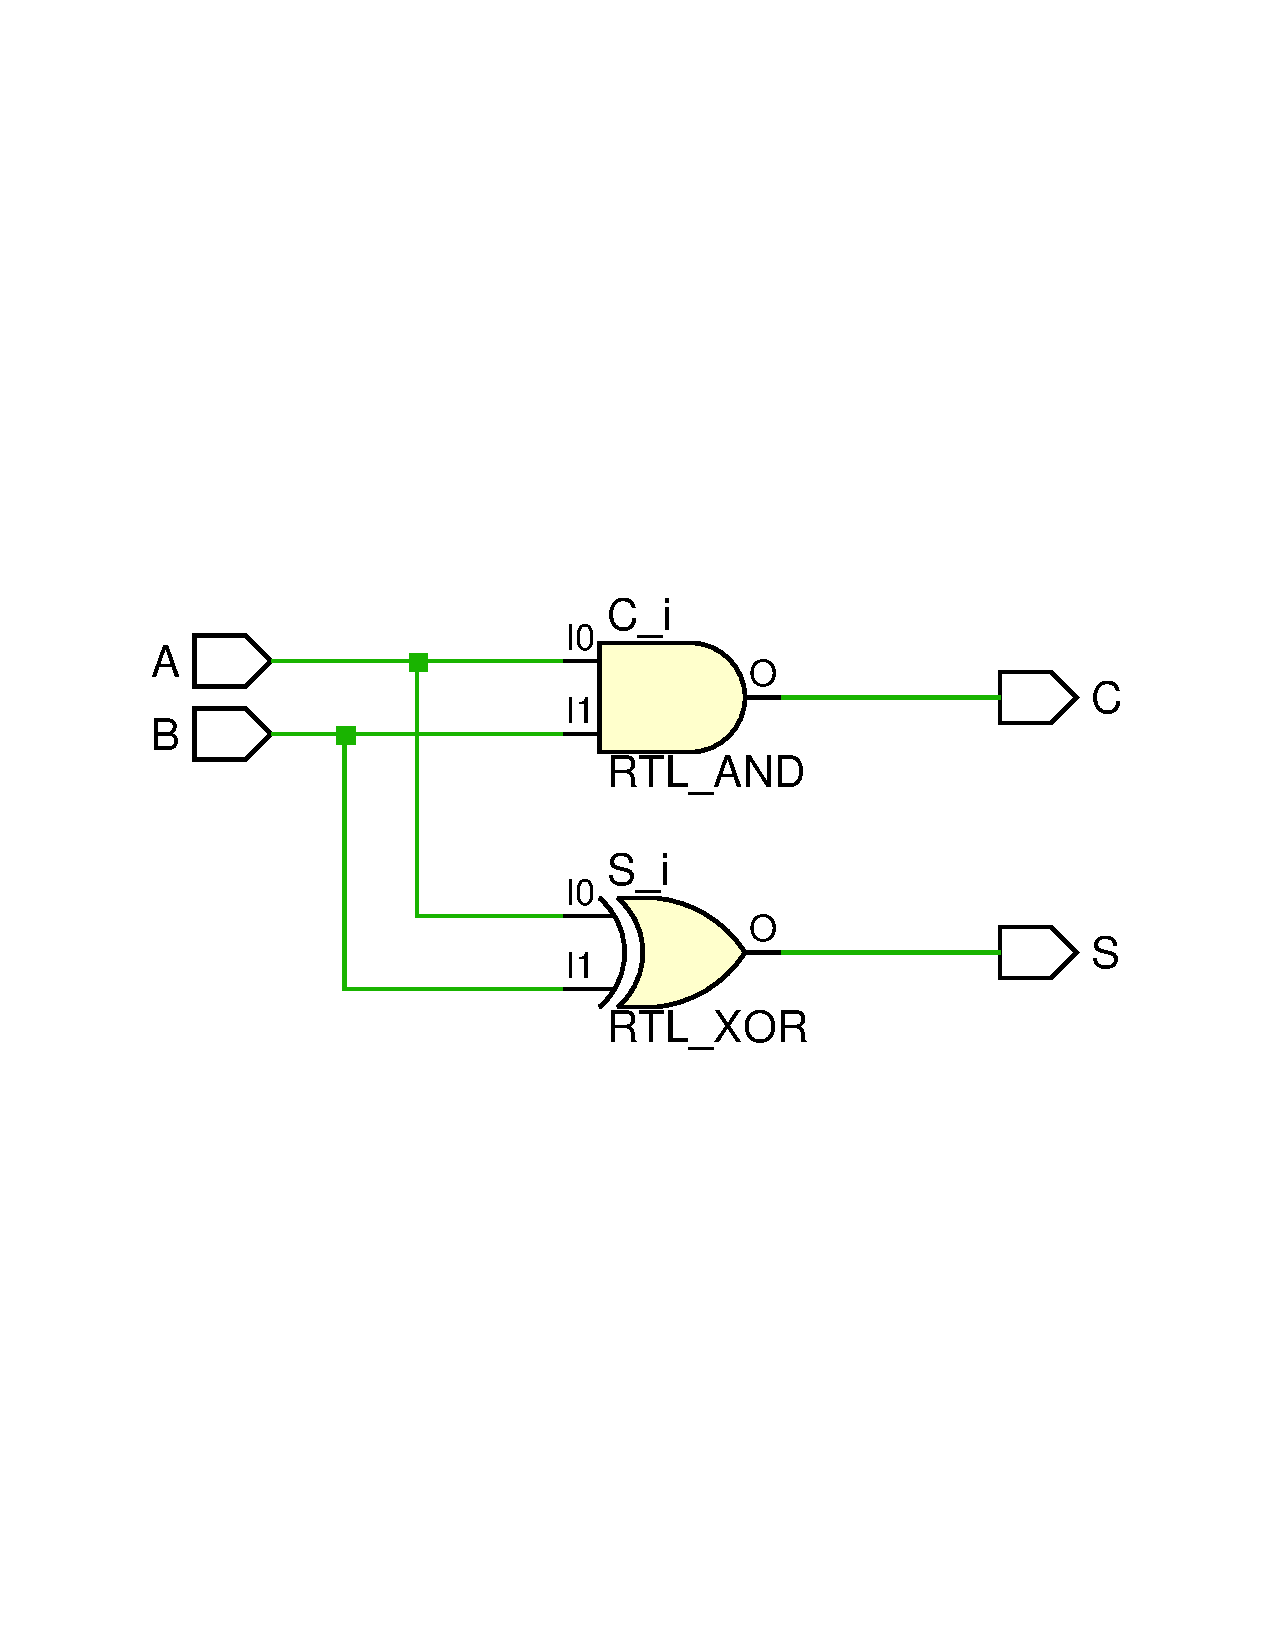
\includegraphics[width=0.5\textwidth]{halfadder_RTL.png}


\end{itemize}
\subsubsection{全加器}

\begin{itemize}
\item
  电路功能:实现将两个输入位和一个进位输入相加,产生一个输出和一个进位输出
\item
  代码设计:
  
  \includegraphics[width=1\textwidth]{fulladder_Code.png}
\item

  RTL分析结果:
  
  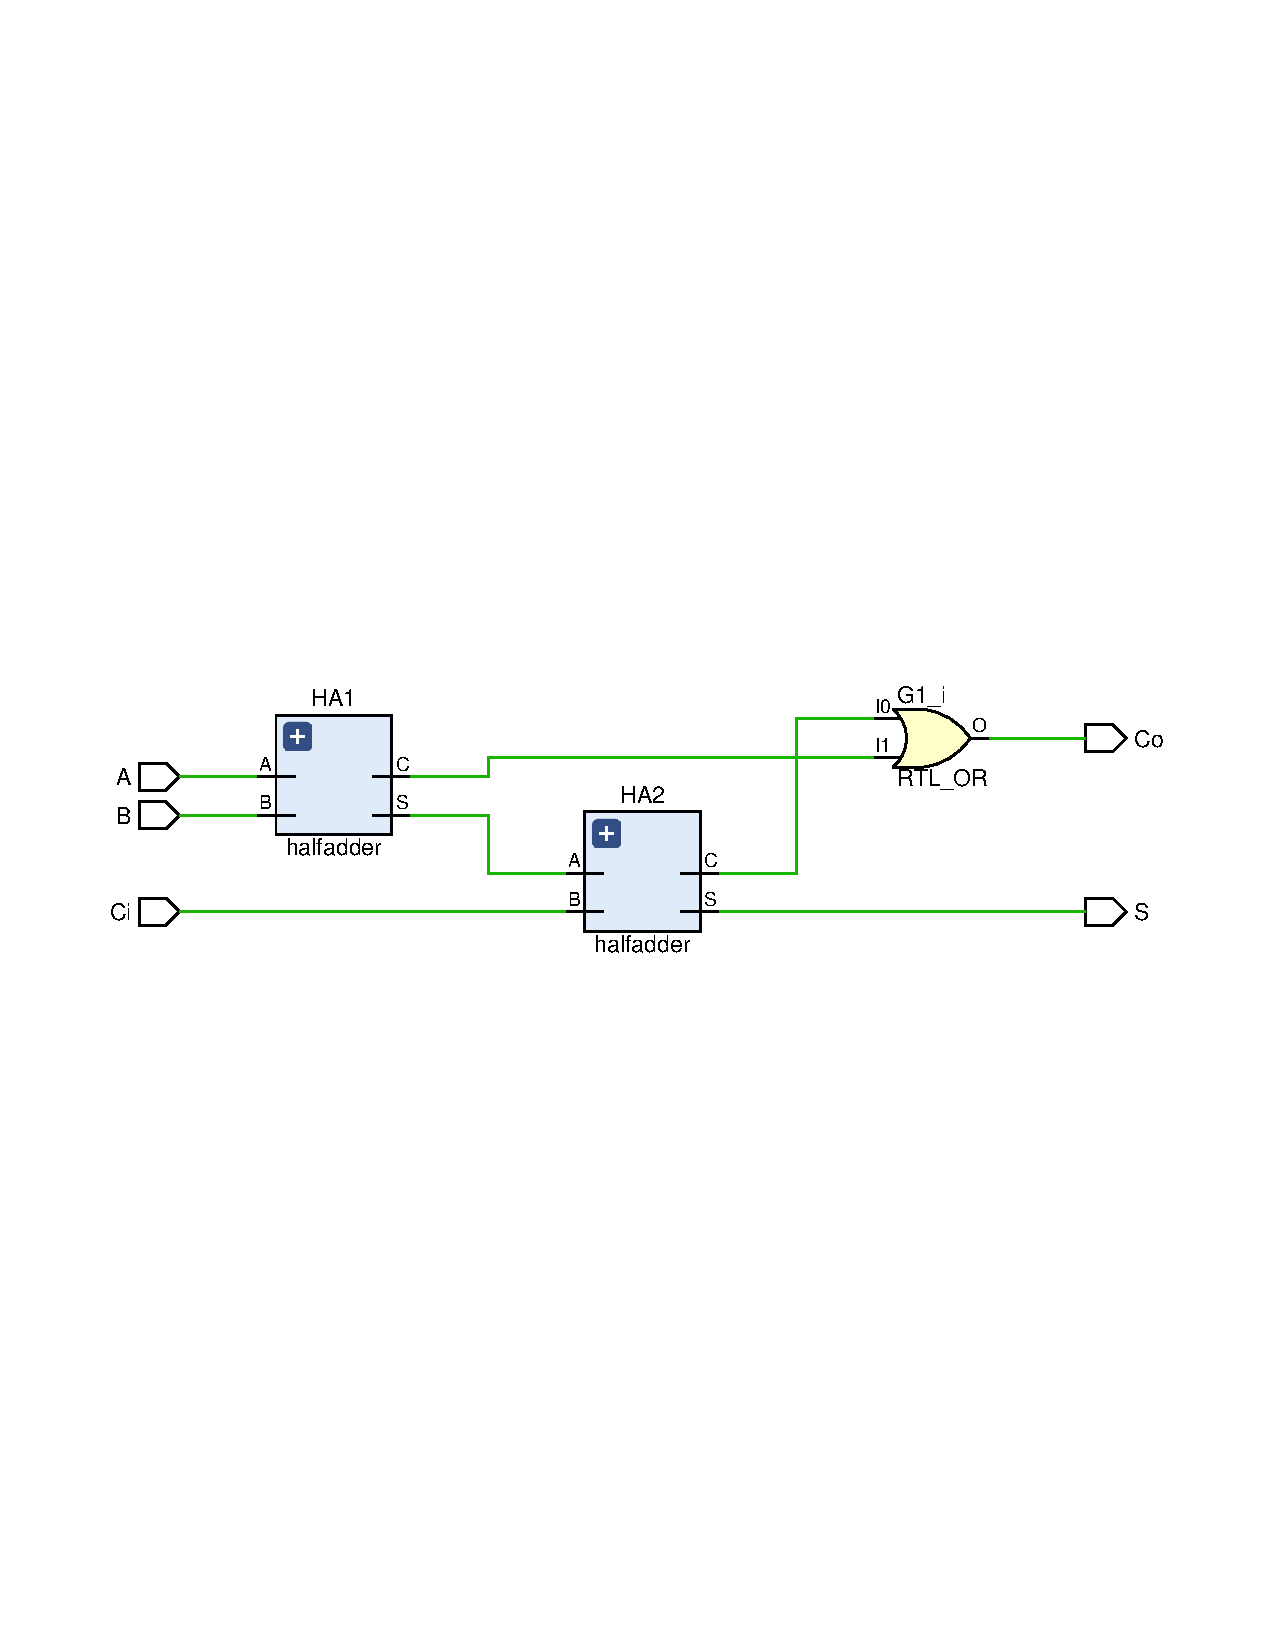
\includegraphics[width=0.8\textwidth]{fulladder_RTL.png}
\item

  Simulation结果:
  
  \includegraphics[width=0.8\textwidth]{fulladder_Simulation.png}
\end{itemize}

\newpage
\subsection{实现2位全加器,并烧录到开发板进行验证}
\subsubsection{实现2位全加器}
\begin{itemize}
\item
  电路功能:实现两个两位二进制数的算术加法运算
\item
  代码设计:
  
  \includegraphics[width=1\textwidth]{2bitadder_Code.png}
\item

  RTL分析结果:
  
  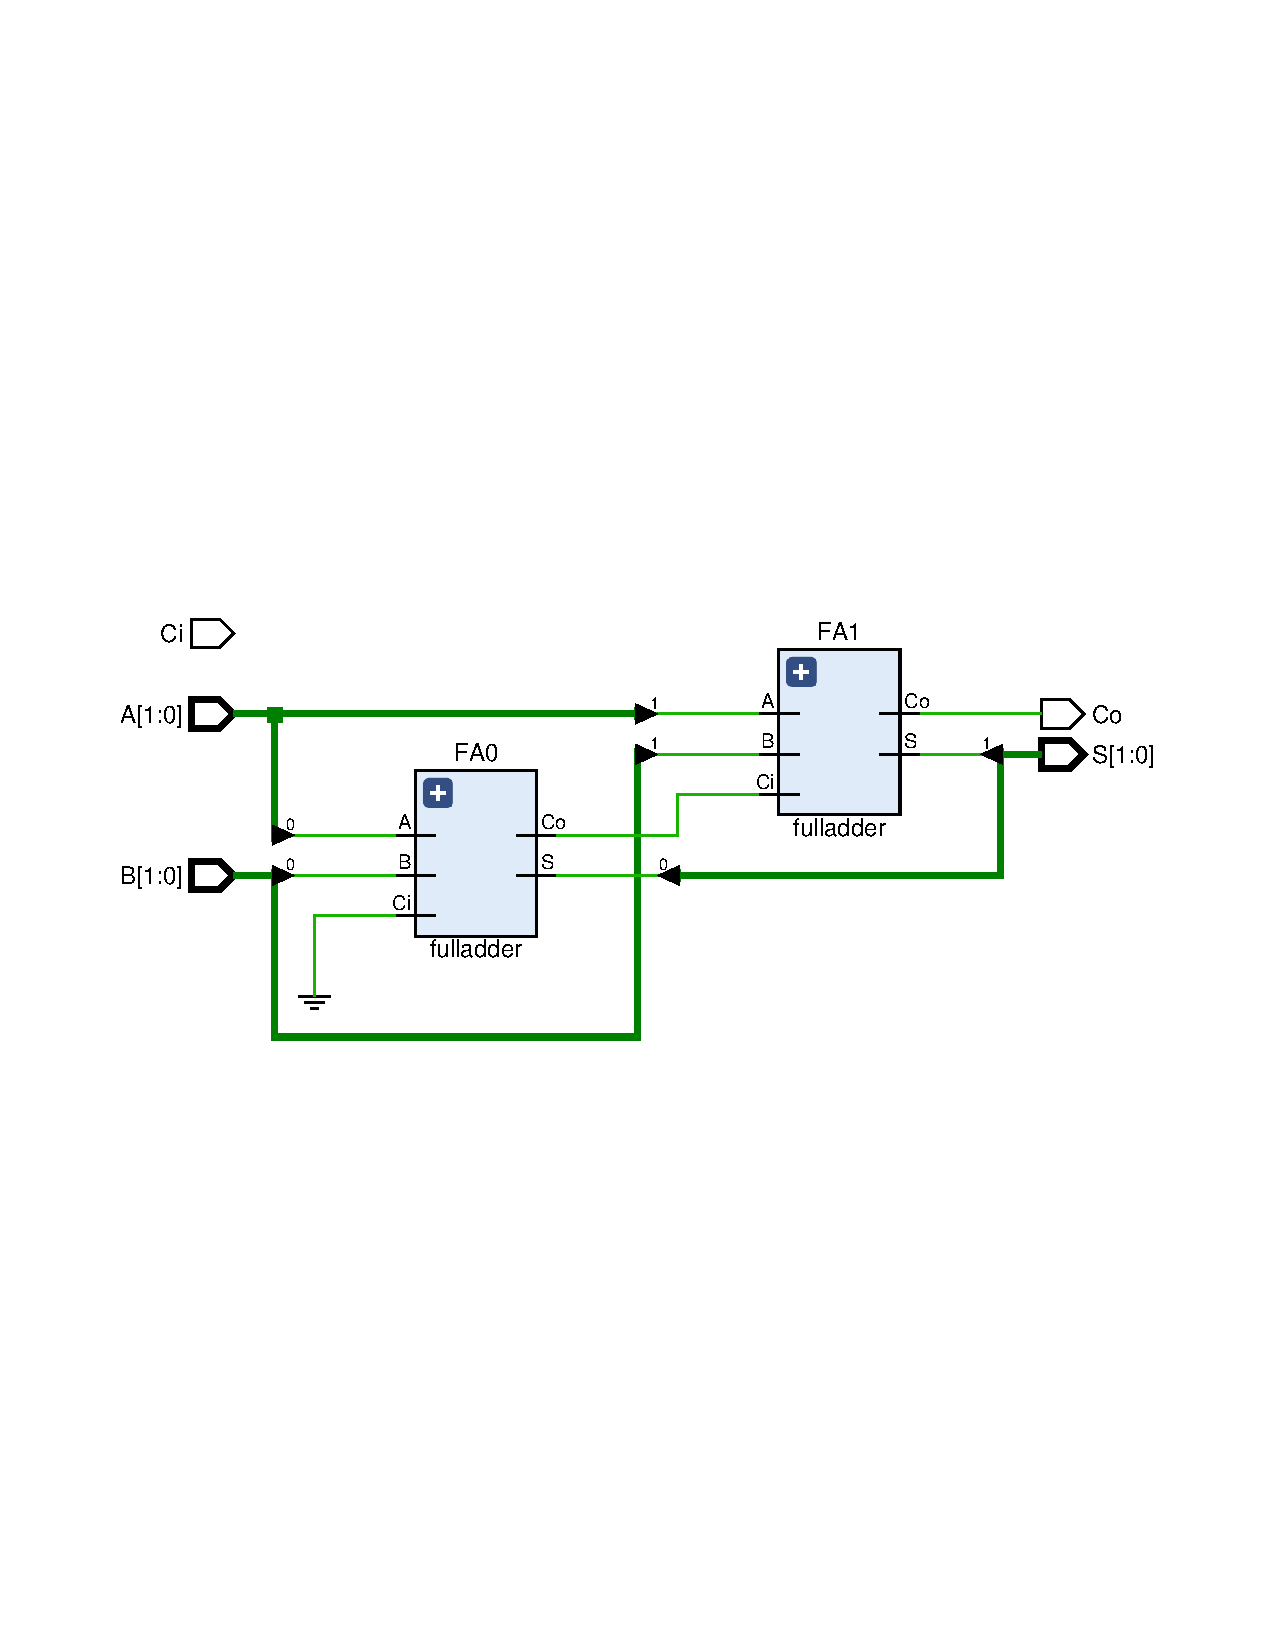
\includegraphics[width=0.8\textwidth]{2bitadder_RTL.png}
\item

  Simulation结果:
  
  \includegraphics[width=0.8\textwidth]{2bitadder_Simulation.png}
\end{itemize}

\subsubsection{将2位全加器烧录}
\paragraph{1. 约束文件}:

用4个拨码开关表示2个加数,1个按键表示最低位进位,3个LED表示二进制输出,1个数码管表示十六进制输出
  
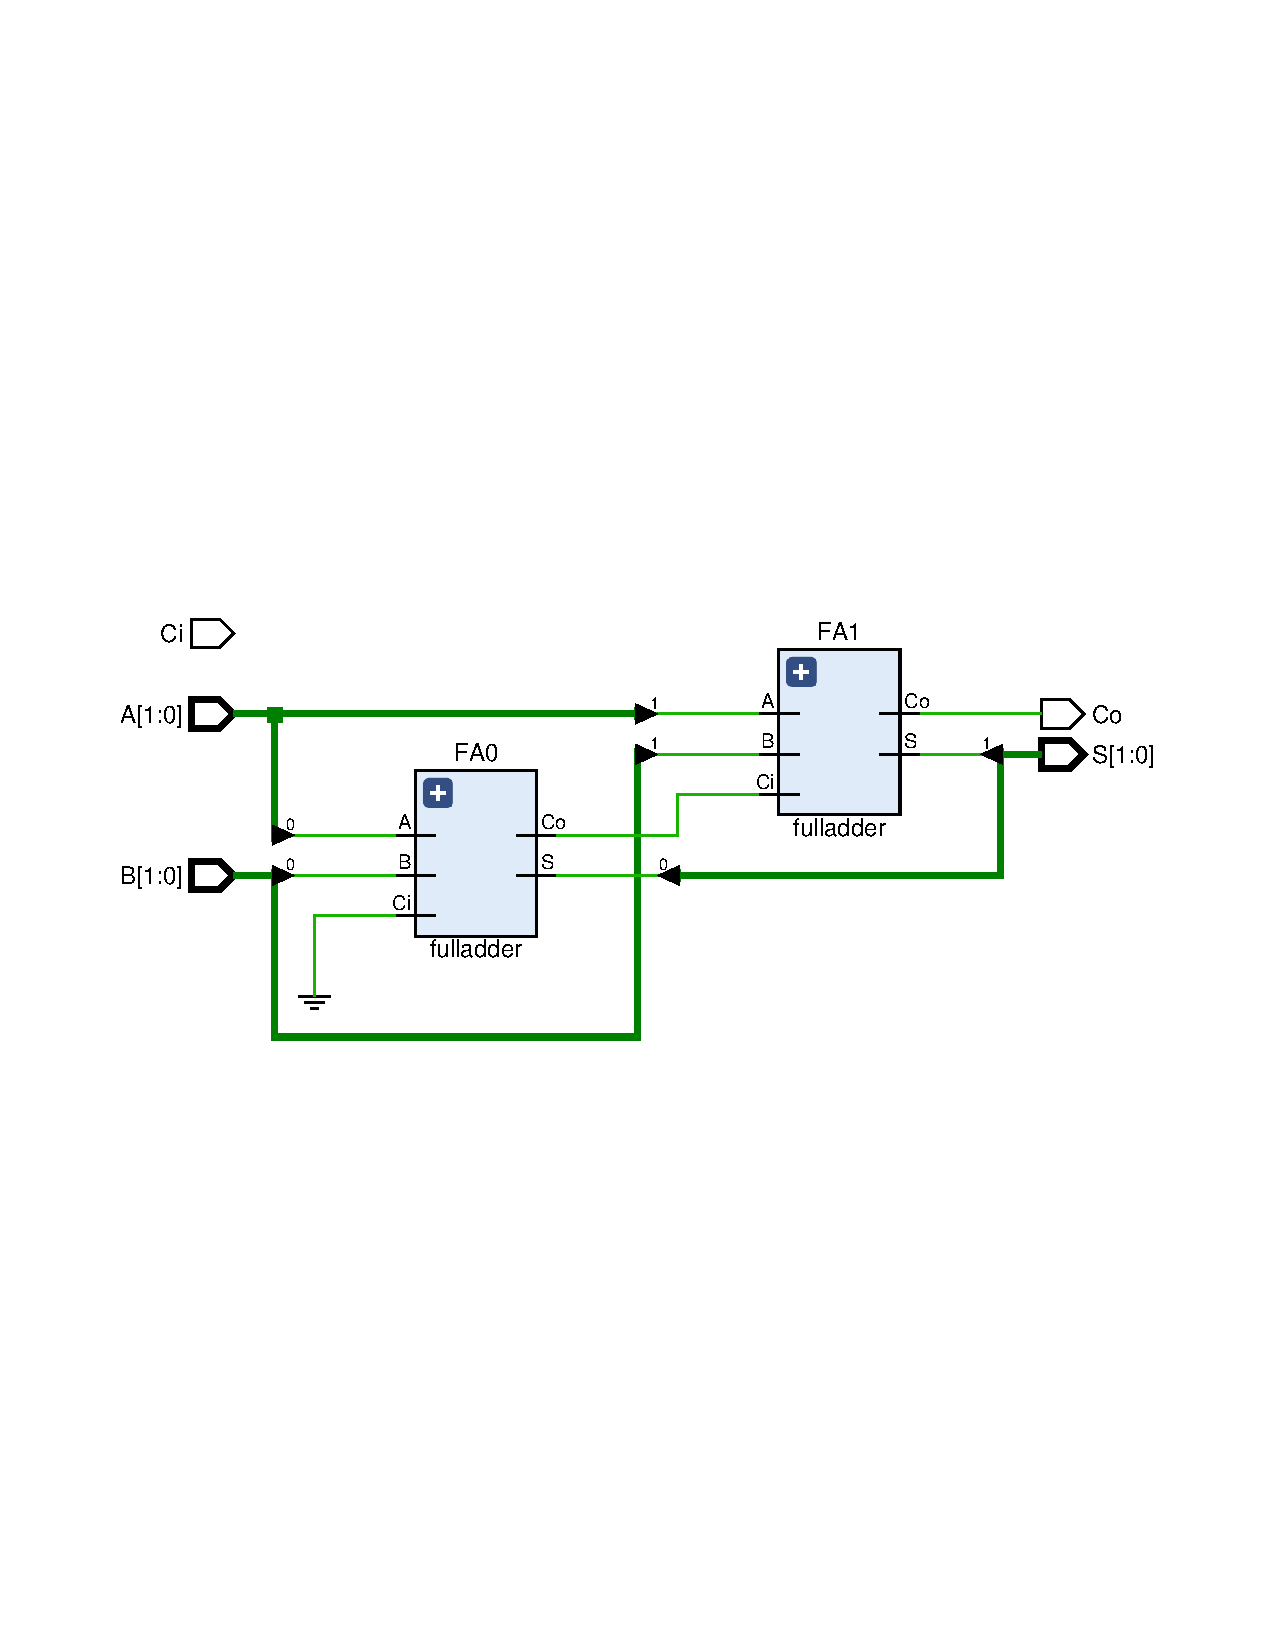
\includegraphics[width=0.8\textwidth]{2bitadder_RTL.png}

  
\paragraph{2. 2位全加器封装模块和EGo1数码管显示模块}:


2位全加器封装模块代码如下,定义了一个名为addr2b\_hex8seg\_EGo1的模块,将两个2位加数A和B进行二进制加法,并将结果通过另一个子模块hex8seg\_EGo1,将加法的输出结果(S和Co)显示在数码管上。

\includegraphics[width=1\textwidth]{2位全加器封装模块.png}
 

EGo1数码管显示模块的代码如下,其是用来控制一个七段数码管显示0到F(十六进制)的数字的。输入S是一个4位的二进制值,根据这个值,代码通过seg\_data\_o\_pin输出对应的数码管编码来显示相应的数字。每个数字或字符对应一个特定的8位编码,这个编码决定了数码管上哪些段应该被点亮。此外,seg\_cs\_pin始终被设定为选中第一个数码管。

\includegraphics[width=0.8\textwidth]{EGo1数码管显示模块.png}

\paragraph{3. RTL分析结果}:

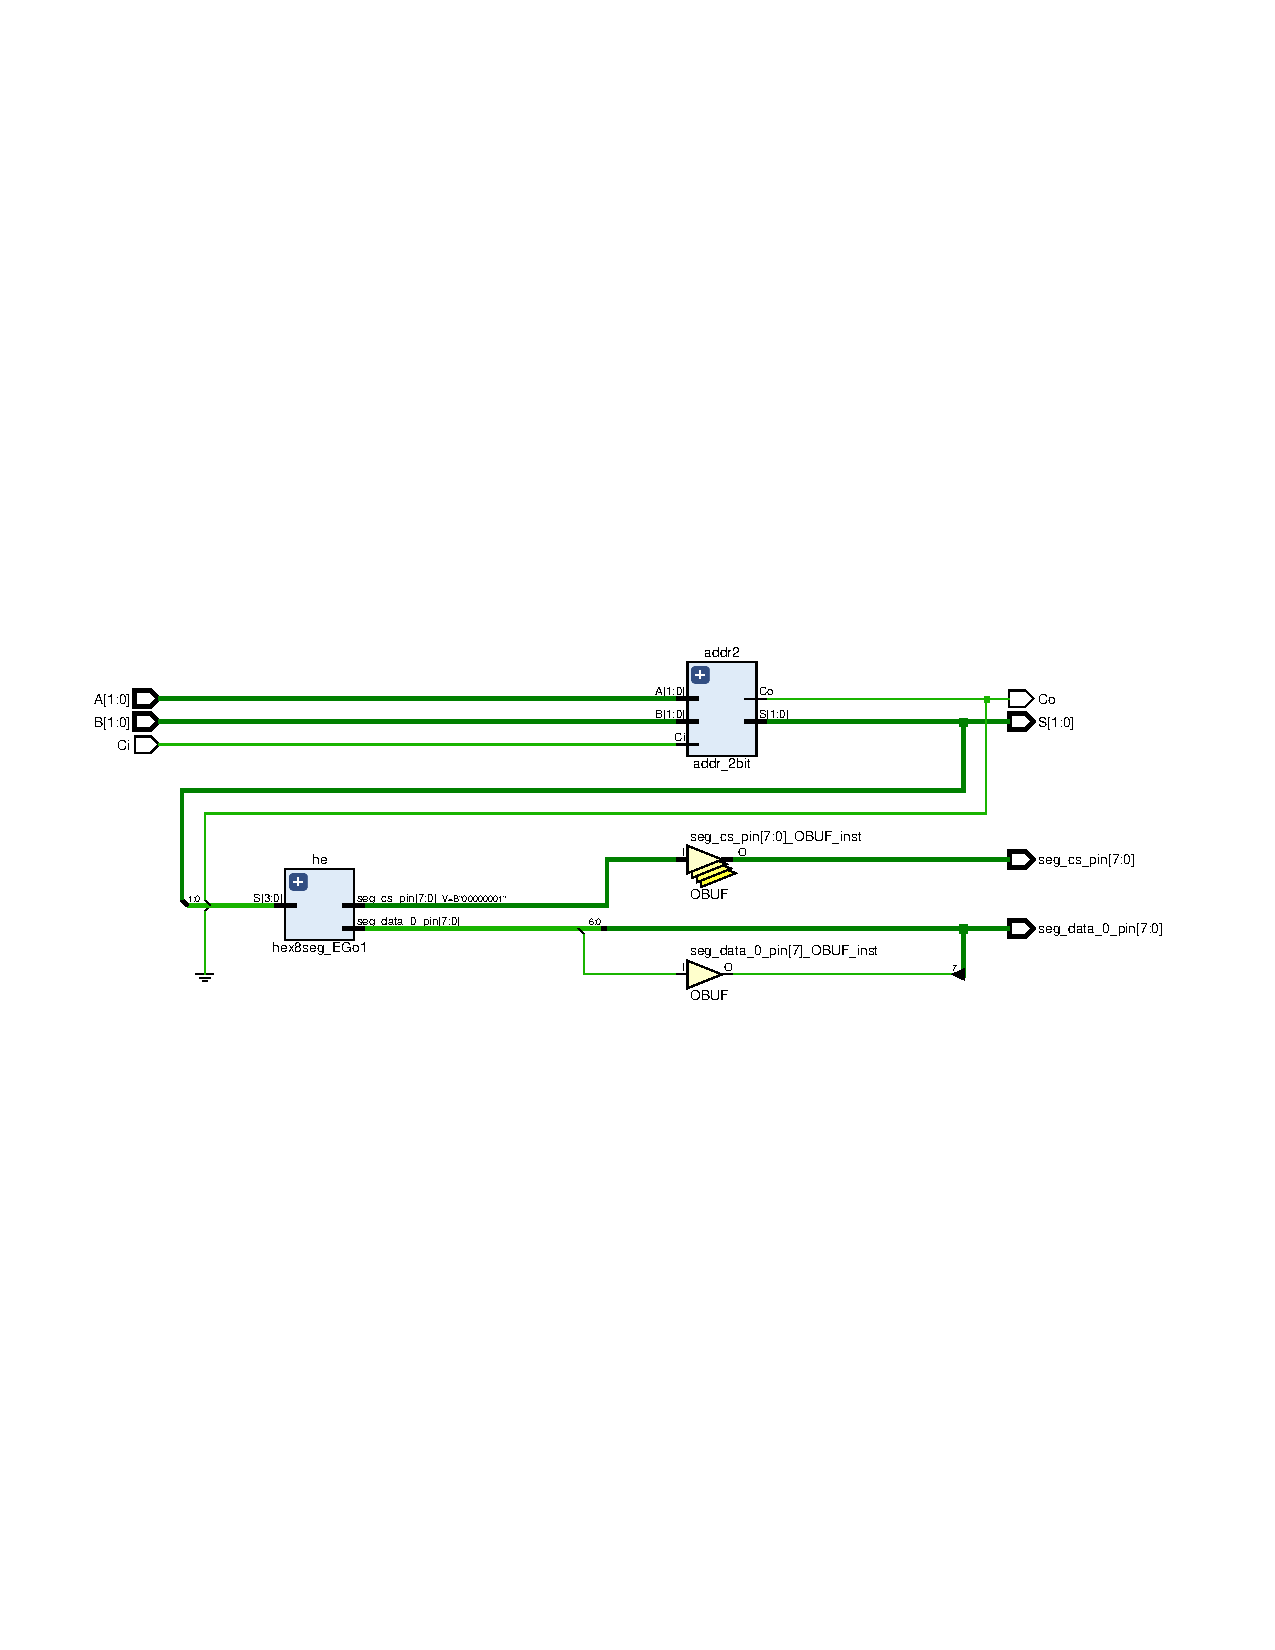
\includegraphics[width=1\textwidth]{ego1_RTL.png}

\paragraph{4. 烧录至开发板进行验证}:


\begin{figure}[!h]
	\centering
	\begin{minipage}{0.49\linewidth}
		\centering
		\includegraphics[width=0.8\textwidth]{板载结果2.jpg}
	\end{minipage}
	\begin{minipage}{0.49\linewidth}
		\centering
		\includegraphics[width=0.8\textwidth]{板载结果3.jpg}
	\end{minipage}
	%\qquad
	%让图片换行,
	\begin{minipage}{0.49\linewidth}
		\centering
		\includegraphics[width=0.8\textwidth]{板载结果5.jpg}

	\end{minipage}
	\begin{minipage}{0.49\linewidth}
		\centering
		\includegraphics[width=0.8\textwidth]{板载结果6.jpg}

	\end{minipage}
\end{figure}


\newpage
\subsection{实现16/32位全加器}

\begin{itemize}
\item
  电路功能:实现实现16位全加器
\item
  代码设计:
    
\qquad addr\_16bit模块是一个典型的多位串行加法器,使用了一系列的全加器(fulladder)实例来逐位计算两个16位数字A和B的和。

\qquad 其中第一个全加器FA0接收最低位和初始进位Cl,而每个随后的全加器接收前一个全加器的进位输出。最后一个全加器FA15的进位输出是Ch,这是整个16位加法的最终进位输出。

\qquad 也就是说每个全加器产生的进位直接传递给下一个全加器的进位输入,形成一个进位链。
  
  \includegraphics[width=0.6\textwidth]{16bitadder_Code.png}
\item

  RTL分析结果:
  
  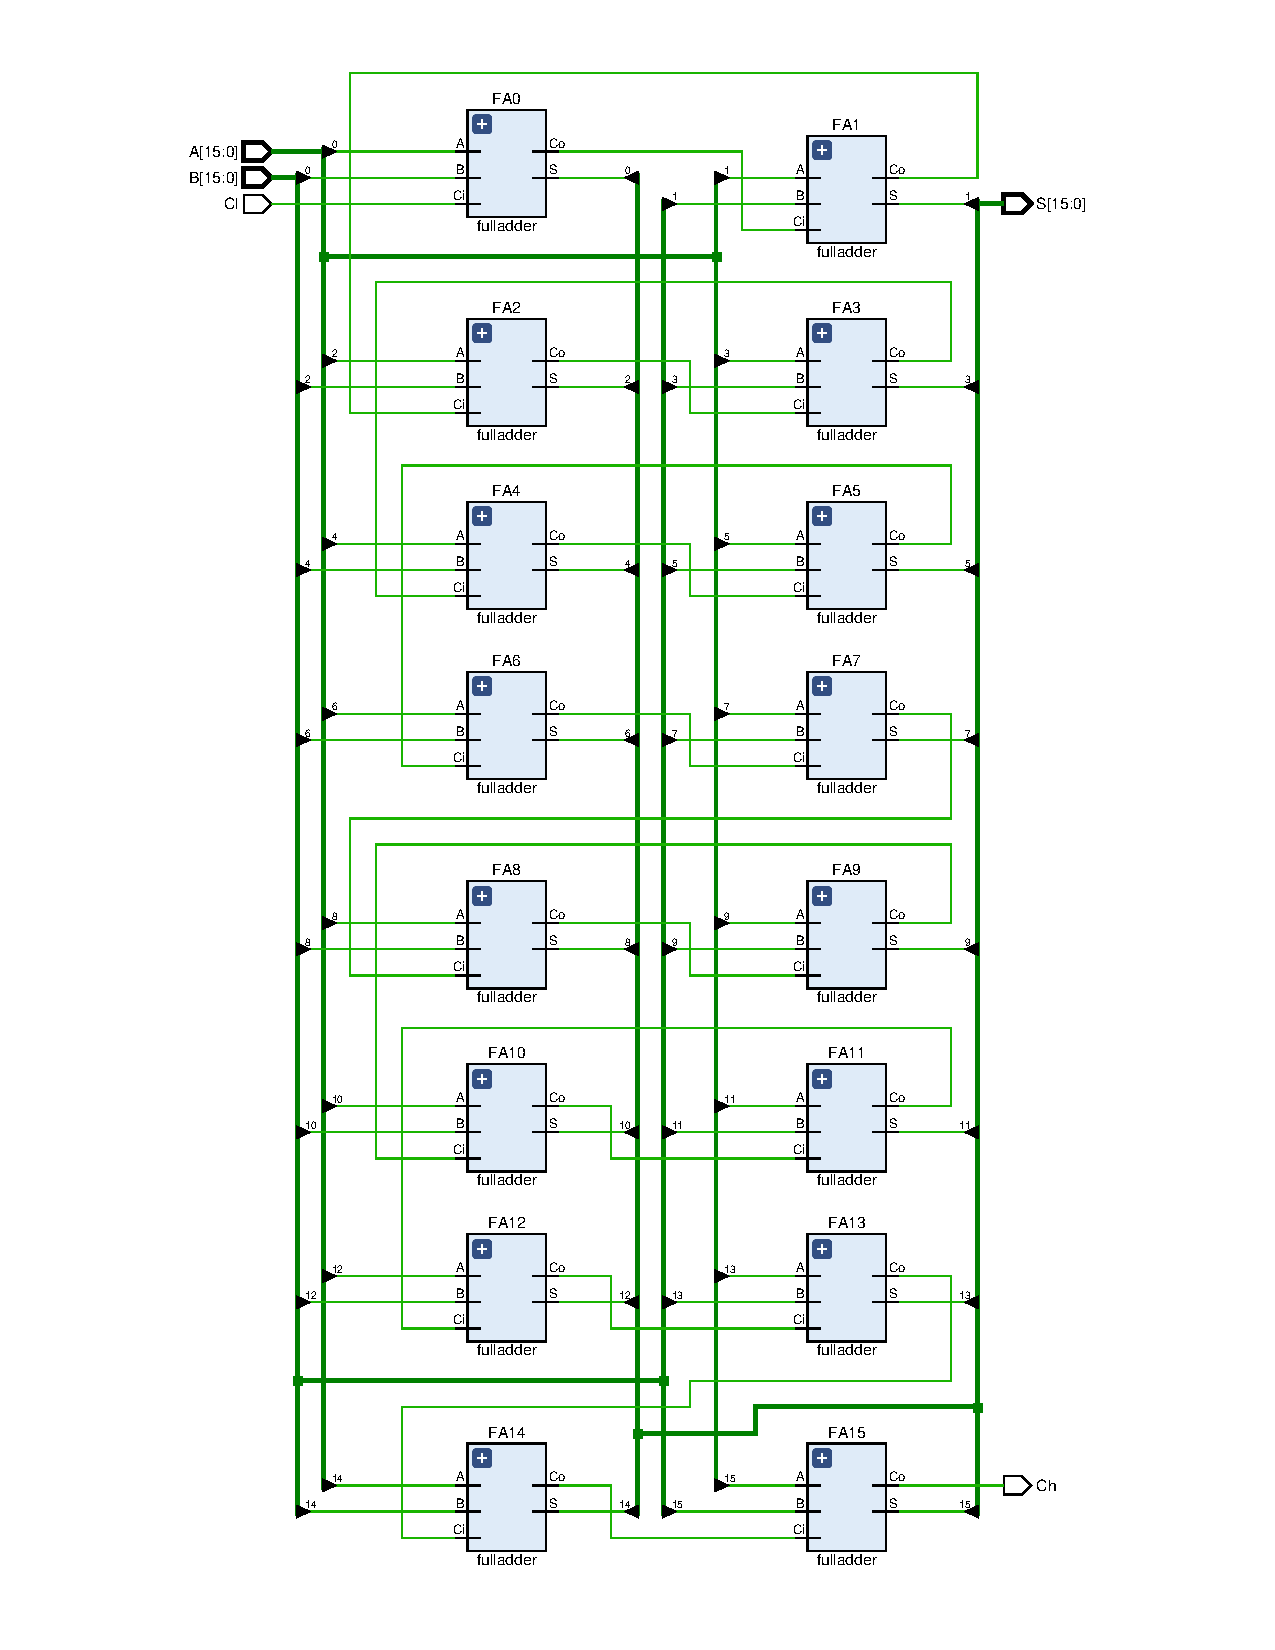
\includegraphics[width=1\textwidth]{16bitadder_RTL.pdf}
\item

  Simulation结果:
  
  \includegraphics[width=1\textwidth]{16bitadder_Simulation.png}
\end{itemize}




\section{调试和心得体会}

在本次实验中,我深刻体会到了数字电路设计的复杂性与挑战性。从设计基本的1位半加器到构建完整的16位全加器,每一步都需要精确的逻辑思考和细致的调试工作。

\subsection{调试过程}

\begin{itemize}
    \item \textbf{代码逻辑错误}:最初在编写16位加法器时,我忽视了进位链的正确传递,导致加法结果不正确。通过反复检查代码和RTL分析生成的图表,我逐步定位到了问题所在,并对进位逻辑进行了调整。


\end{itemize}


\subsection{心得体会}

\begin{itemize}
    \item \textbf{理论与实践的结合}:虽然理论知识为我们提供了设计的基础,但实际操作时仍然需要根据具体情况进行调整。每一次的编程和调试都让我对Verilog语言和FPGA的实际应用有了更深刻的理解。
    
    \item \textbf{细节的重要性}:在数字电路设计中,每一个小小的逻辑错误都可能导致整个系统的失败。我学会了如何更加注意信号的精确控制和逻辑的正确设置。
    
\end{itemize}


本次实验,我深入学习了Verilog编程,设计了从1位到16位的加法器,并通过Vivado平台进行了详细的仿真和分析。实验涵盖了从基本的半加器和全加器到复杂的16位加法器的设计和测试,包括在FPGA开发板上的实际烧录和验证。这一过程不仅增强了我对数字逻辑和硬件设计的理解,还锻炼了我解决问题的能力,尤其是在硬件配置和调试方面。通过这次实践,我意识到理论学习与实际操作之间的密切联系,并且学会了如何分析硬件设计的逻辑错误,与解决问题的方法。

\end{document}
